\section{独立随机变量}
\label{sec:rvc-independence}

图~\ref{fig:rvc-same-marginals}(b)的表是用边缘“乘出来”的。什么时候真实的联合分布恰好就是这张乘积表？第~\ref{chap:classical-probability}章说过，两个事件独立，是指它们同时发生的概率等于各自概率之积。把这一要求加到由两个随机变量生成的每一对事件上，就得到随机变量的独立。

\paragraph{联合分布分解为边缘乘积}
第一台传感器读数落在某个范围，是一个事件；第二台读数落在某个范围，是另一个事件。如果知道其中一个的结果从来不改变另一个的概率，就说两台读数互不提供信息。下面的定义只对区间提出要求，区间可以是单点、有界区间或半直线。

\begin{definition}[独立随机变量]
\label{def:rvc-independence}
若对实数轴上的任意区间$A$和$B$都有
\begin{equation}
 \mathbb{P}(X\in A,\,Y\in B)=\mathbb{P}(X\in A)\,\mathbb{P}(Y\in B),
 \label{eq:rvc-independence}
\end{equation}
则称$X$与$Y$是\term{独立随机变量}（independent random variables），简称$X$与$Y$独立。
\end{definition}

取$A=(-\infty,x]$，$B=(-\infty,y]$，式~\eqref{eq:rvc-independence}给出$F_{X,Y}(x,y)=F_X(x)F_Y(y)$。反过来，若联合分布函数对一切$(x,y)$都分解为边缘分布函数之积，由式~\eqref{eq:rvc-rectangle}，每个半开矩形的概率都分解，独立性的其余情形可由这些矩形取极限得到，这一步留到第~\ref{chap:probability-spaces}章。实际计算中更常用的是下面针对概率表和密度的判别。

\begin{theorem}[独立性的判别]
\label{thm:rvc-independence-criterion}
\begin{enumerate}
 \item 若$X,Y$都只取有限个或可数个值，则$X$与$Y$独立，当且仅当对一切$x,y$，
 \begin{equation}
 p_{X,Y}(x,y)=p_X(x)\,p_Y(y).
 \label{eq:rvc-independence-pmf}
 \end{equation}
 \item 若$(X,Y)$有联合密度，$X,Y$分别有边缘密度$f_X,f_Y$，则$X$与$Y$独立，当且仅当乘积$f_X(x)f_Y(y)$也是$(X,Y)$的联合密度。特别地，若联合密度可以写成$f_{X,Y}(x,y)=g(x)h(y)$，其中$g,h$非负，则$X$与$Y$独立，并且
 \begin{equation}
 f_X=\frac{g}{\int g},\qquad f_Y=\frac{h}{\int h}.
 \label{eq:rvc-factorization}
 \end{equation}
\end{enumerate}
\end{theorem}

\begin{proof}
先看概率表。若$X,Y$独立，取单点区间$A=[x,x]$、$B=[y,y]$，式~\eqref{eq:rvc-independence}就是式~\eqref{eq:rvc-independence-pmf}。反过来，若式~\eqref{eq:rvc-independence-pmf}成立，对任意区间$A,B$，由式~\eqref{eq:rvc-joint-pmf-event}，
\[
 \mathbb{P}(X\in A,\,Y\in B)=\sum_{x\in A}\sum_{y\in B}p_X(x)\,p_Y(y).
\]
各项非负，二重和可以按任意顺序计算，先对$y$求和，得到
\[
 \sum_{x\in A}p_X(x)\sum_{y\in B}p_Y(y)=\mathbb{P}(X\in A)\,\mathbb{P}(Y\in B).
\]

再看密度。若$f_Xf_Y$是联合密度，对矩形$A\times B$，被积函数是$x$的函数与$y$的函数之积，累次积分分开计算：
\[
 \mathbb{P}(X\in A,\,Y\in B)=\int_{A}f_X(x)\,\mathrm{d}x\int_{B}f_Y(y)\,\mathrm{d}y=\mathbb{P}(X\in A)\,\mathbb{P}(Y\in B).
\]
无界区间按非负函数积分取极限理解。反过来，若$X,Y$独立，对每个矩形$R=A\times B$，
\[
 \iint_{R}f_X(x)f_Y(y)\,\mathrm{d}x\,\mathrm{d}y=\mathbb{P}(X\in A)\,\mathbb{P}(Y\in B)=\mathbb{P}\bigl((X,Y)\in R\bigr),
\]
这正是定义~\ref{def:rvc-joint-density}对联合密度的要求。

最后设$f_{X,Y}=gh$。由式~\eqref{eq:rvc-marginal-density}，$f_X(x)=g(x)\int h$，$f_Y(y)=h(y)\int g$；联合密度的总积分为$1$，即$\int g\int h=1$。于是
\[
 f_X(x)f_Y(y)=g(x)h(y)\int g\int h=g(x)h(y)=f_{X,Y}(x,y),
\]
由已证部分，$X$与$Y$独立，式~\eqref{eq:rvc-factorization}也同时得到。
\end{proof}

第二条说“乘积也是联合密度”，而不说“联合密度处处等于乘积”，是因为密度不唯一。把联合密度在一条直线上的值改掉，任何矩形上的积分都不变，改过的函数仍是联合密度，却可能在这条直线上不等于乘积。第~\ref{chap:probability-spaces}章会用“除去面积为零的集合”统一处理这类差别。

\paragraph{判别的例子}
两颗均匀骰子的点数$X_1,X_2$独立：每对点数的概率$1/36$恰好等于$\frac16\cdot\frac16$。同一试验中的$X$与$M$却不独立。由图~\ref{fig:rvc-dice-map}，
\[
 p_{X,M}(2,1)=0,\qquad p_X(2)\,p_M(1)=\frac16\cdot\frac1{36}>0 .
\]
只要找到一个格子不满足式~\eqref{eq:rvc-independence-pmf}，就足以否定独立。

两台传感器也不独立：$p_{X,Y}(0,2)=0$，而$p_X(0)p_Y(2)=0.09$。图~\ref{fig:rvc-same-marginals}(b)那张乘积表描述的才是“边缘相同而相互独立”的两台传感器。对照两张表可以看到，独立是对整张表的要求，九个格子都要分解。

连续情形里，单位正方形上的密度$f(x,y)=4xy$可以写成$(2x)(2y)$，所以两个分量独立，边缘密度都是$2t$，$0\leq t\leq 1$。三角形模型则不独立，理由可以直接从图上读出。取$A=[0,1/2)$，$B=(1/2,1]$，矩形$A\times B$整个落在三角形外，所以$\mathbb{P}(X<1/2,\,Y>1/2)=0$。而由两个边缘密度，
\[
 \mathbb{P}(X<\tfrac12)=\int_{0}^{1/2}2x\,\mathrm{d}x=\tfrac14,\qquad
 \mathbb{P}(Y>\tfrac12)=\int_{1/2}^{1}2(1-y)\,\mathrm{d}y=\tfrac14,
\]
乘积为$1/16\neq 0$。

这个论证给出一条常用的经验：若$X,Y$独立，联合质量只能分布在“$X$可能取的值”与“$Y$可能取的值”组成的乘积形区域上。三角形、圆盘这类不是乘积形的区域上的均匀分布，分量一定不独立。反之，区域是乘积形并不保证独立，图~\ref{fig:rvc-fgm}中$\theta\neq 0$的密度就是反例。

判别定理回答的是“给定联合分布，分量是否独立”。实际建模时常常反过来：两颗骰子分别掷出、两台仪器各自供电，物理上互不影响，于是\emph{假定}它们独立，再用定理~\ref{thm:rvc-independence-criterion}由边缘写出联合分布。这一假定是否合适，要回到试验本身判断；一旦假定错了，例如两台传感器其实受同一股气流影响，按乘积表算出的$\mathbb{P}(X=Y)=0.34$就会低估真实的$0.60$。

\paragraph{多个随机变量的独立}
传感器不止两台时，要求每一组读数范围的联合概率都分解。设$X_1,\dots,X_d$定义在同一样本空间上。若对任意区间$A_1,\dots,A_d$都有
\begin{equation}
 \mathbb{P}(X_1\in A_1,\dots,X_d\in A_d)=\prod_{i=1}^{d}\mathbb{P}(X_i\in A_i),
 \label{eq:rvc-mutual-independence}
\end{equation}
则称$X_1,\dots,X_d$\term{相互独立}（mutually independent）。取某些$A_i$为整个实数轴，这些因子变成$1$，所以任意一部分变量也相互独立。概率表和密度的判别与定理~\ref{thm:rvc-independence-criterion}相同：联合质量函数或联合密度分解为$d$个边缘之积。

只要求每两个变量独立，称为\term{两两独立}（pairwise independent），这比相互独立弱。令$X,Y$独立，各以概率$1/2$取$1$或$-1$，再令$Z=XY$。$(X,Y,Z)$只有四种等可能的取值，即图~\ref{fig:rvc-pairwise}中的四个实心点。

\begin{BookInlineFigure}
  \centering
  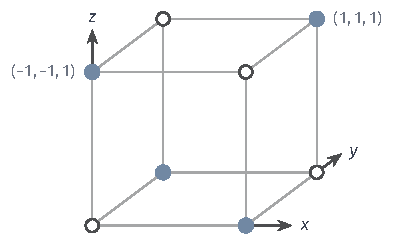
\includegraphics[width=67mm]{figures/07-probability/01-elementary-probability/tikz/rvc-pairwise/figure.pdf}
  \caption{两两独立但不相互独立。$X,Y$是独立的等可能符号，$Z=XY$。立方体八个角中，四个实心点满足$z=xy$，各有概率$1/4$；四个空心点的概率为零。从任一坐标方向把立方体压到一个面上，四个实心点恰好落在该面的四个角，每角$1/4$。}
  \label{fig:rvc-pairwise}
\end{BookInlineFigure}

先验证$X$与$Z$独立。$Z$等可能取$\pm1$。对任意$x,z\in\{1,-1\}$，事件$\{X=x,Z=z\}$就是$\{X=x,Y=xz\}$，于是
\[
 \mathbb{P}(X=x,\,Z=z)=\mathbb{P}(X=x)\,\mathbb{P}(Y=xz)=\tfrac14=\mathbb{P}(X=x)\,\mathbb{P}(Z=z).
\]
同理$Y$与$Z$独立，$X$与$Y$本来独立。三者却不相互独立：
\[
 \mathbb{P}(X=1,\,Y=1,\,Z=-1)=0\neq\tfrac18 .
\]
知道$X$和$Y$以后，$Z$完全确定；而单独知道其中任一个，对$Z$没有任何信息。

\paragraph{独立变量的函数}
传感器读数独立时，把读数换算成温度、取平方或截断，结果仍应独立。下面在概率表的情形证明这一点。设$X,Y$只取有限个或可数个值且独立，$g,h$是实函数。对任意区间$A,B$，令$G=\{x:g(x)\in A\}$，$H=\{y:h(y)\in B\}$，则
\[
 \begin{aligned}
 \mathbb{P}\bigl(g(X)\in A,\,h(Y)\in B\bigr)&=\sum_{x\in G}\sum_{y\in H}p_X(x)\,p_Y(y)\\
 &=\mathbb{P}\bigl(g(X)\in A\bigr)\,\mathbb{P}\bigl(h(Y)\in B\bigr).
 \end{aligned}
\]
所以$g(X)$与$h(Y)$独立。有密度时，集合$G,H$可能不再是区间，同样的结论需要第~\ref{chap:probability-spaces}章对一般集合的处理，这里直接使用。多个变量时结论同样成立：相互独立的变量分成互不相交的几组，各组的函数仍相互独立，例如$X_1+X_2$与$X_3^{2}$独立。

\paragraph{联合分布下的期望}
独立性最常用的推论是乘积的期望可以分开计算。先需要知道怎样对联合分布求期望。第~\ref{chap:random-variable-moments}章对一元情形说明，计算$\mathbb{E}[g(X)]$不必先求$g(X)$的分布。二元情形同样如此：在求和或积分绝对收敛时，
\begin{equation}
 \mathbb{E}\bigl[\varphi(X,Y)\bigr]=\sum_{x,y}\varphi(x,y)\,p_{X,Y}(x,y)
 \quad\text{或}\quad
 \iint\varphi(x,y)\,f_{X,Y}(x,y)\,\mathrm{d}x\,\mathrm{d}y .
 \label{eq:rvc-joint-expectation}
\end{equation}
概率表的情形，把取值对按$\varphi(x,y)$的值分组，同组质量之和就是$\varphi(X,Y)$取该值的概率，于是左右两边是同一个和的两种排列。密度的情形，$\varphi(X,Y)$可能既无概率表也无密度，它的期望及上式的证明要用第~\ref{chap:probability-spaces}章的积分，这里把上式当作计算规则使用。$d$维时把二元和、二重积分换成$d$元和、$d$重积分。

\begin{theorem}[独立变量乘积的期望]
\label{thm:rvc-product-expectation}
设$X$与$Y$独立，$\mathbb{E}\lvert g(X)\rvert<\infty$，$\mathbb{E}\lvert h(Y)\rvert<\infty$。则$g(X)h(Y)$的期望存在，并且
\begin{equation}
 \mathbb{E}\bigl[g(X)h(Y)\bigr]=\mathbb{E}\bigl[g(X)\bigr]\,\mathbb{E}\bigl[h(Y)\bigr].
 \label{eq:rvc-product-expectation}
\end{equation}
\end{theorem}

\begin{proof}
在概率表的情形，由定理~\ref{thm:rvc-independence-criterion}，联合质量等于$p_X(x)p_Y(y)$。先检查绝对收敛：非负项的二重和可以先对$y$求和，
\[
 \sum_{x,y}\lvert g(x)\rvert\,\lvert h(y)\rvert\,p_X(x)\,p_Y(y)
 =\Bigl(\sum_{x}\lvert g(x)\rvert p_X(x)\Bigr)\Bigl(\sum_{y}\lvert h(y)\rvert p_Y(y)\Bigr)<\infty .
\]
因此由式~\eqref{eq:rvc-joint-expectation}，$\mathbb{E}[g(X)h(Y)]$存在。绝对收敛的二重和同样可以先对$y$求和，去掉绝对值重复上面的计算，就得到式~\eqref{eq:rvc-product-expectation}。在密度的情形，取$f_Xf_Y$为联合密度，把求和换成积分：先对非负的$\lvert g(x)h(y)\rvert f_X(x)f_Y(y)$做累次积分，确认积分有限，再按绝对可积函数的累次积分规则分开计算。
\end{proof}

可积条件的作用是保证求和与积分的次序可以交换；只有两个期望都有限，右边的乘积才有意义。例如两颗骰子的点数之积，期望为$(7/2)^{2}=49/4$；$f=4xy$的模型中，
\[
 \mathbb{E}[XY]=\int_{0}^{1}\!\!\int_{0}^{1}xy\cdot 4xy\,\mathrm{d}x\,\mathrm{d}y=4\cdot\frac13\cdot\frac13=\frac49 ,
\]
恰好是$\mathbb{E}[X]^{2}=(2/3)^{2}$。

定理也可以反过来用于否定独立。三角形模型中$\mathbb{E}[X]=2/3$，$\mathbb{E}[Y]=1/3$，而
\[
 \mathbb{E}[XY]=\int_{0}^{1}\!\!\int_{0}^{x}2xy\,\mathrm{d}y\,\mathrm{d}x=\int_{0}^{1}x^{3}\,\mathrm{d}x=\frac14\neq\frac29 .
\]
但等式~\eqref{eq:rvc-product-expectation}只对一对特定的函数成立时，并不能推出独立，第~\ref{sec:rvc-moments}节会给出反例。

\paragraph{独立同分布}
重复试验的标准模型是：每次试验在相同条件下进行，各次结果互不影响。用随机变量写出来，就是下面的两个要求同时成立。若$X_1,\dots,X_n$相互独立，并且具有同一个分布$P$，则称它们\term{独立同分布}（independent and identically distributed），简记为i.i.d.，并写
\begin{equation}
 X_1,\dots,X_n\overset{\text{i.i.d.}}{\sim}P .
 \label{eq:rvc-iid}
\end{equation}
由定理~\ref{thm:rvc-independence-criterion}，它们的联合质量函数或联合密度是同一个边缘的$n$次乘积，例如$\prod_{i=1}^{n}p(x_i)$。

“同分布”只约束每个分量各自的规律，“独立”只约束分量之间的关系，两者谁也推不出谁。图~\ref{fig:rvc-iid}用两颗骰子说明三种情况。(a)两颗骰子独立掷出，$36$个格点各有$1/36$，两项都满足。(b)令$X_2=X_1$，两个分量同分布，但质量全在对角线上，不独立。(c)$X_1$是骰子点数，$X_2$是独立抛出的均匀硬币，记正面为$1$，两者独立但分布不同。

\begin{BookInlineFigure}
  \centering
  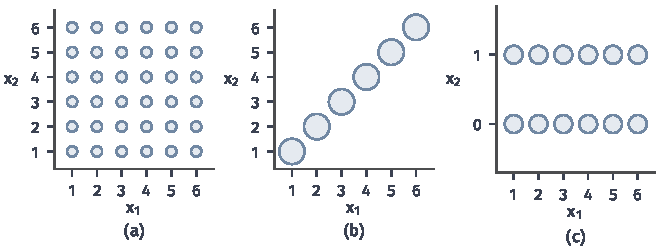
\includegraphics[width=112mm]{figures/07-probability/01-elementary-probability/matplotlib/rvc-iid/figure.pdf}
  \caption{独立与同分布是两项不同的要求，圆的面积正比于联合质量。(a)两颗独立的均匀骰子，每点$1/36$。(b)$X_2=X_1$，对角线上每点$1/6$：同分布，不独立。(c)骰子点数$X_1$与独立的均匀硬币$X_2\in\{0,1\}$，每点$1/12$：独立，不同分布。}
  \label{fig:rvc-iid}
\end{BookInlineFigure}

在(b)中，两次“试验”其实只做了一次，第二个数只是抄写第一个；在(c)中，两次试验互不影响，但做的不是同一种试验。只有(a)对应“同一试验独立重复两次”。后面讨论样本平均为什么随次数增加而稳定时，两项要求分别承担不同作用：同分布保证每次平均的是同一个量，独立保证波动能互相抵消，见第~\ref{chap:laws-of-large-numbers}章。
